\documentclass{beamer}
\usepackage{fancyvrb}
\usepackage{hyperref}
\usepackage{alltt}
\usepackage{graphicx}
\newcommand{\sect}[1]{
\section{#1}
\begin{frame}[fragile]\frametitle{#1}
}

\newtheorem{theo}{Theorem}[section]

\newcommand{\myfig}[1]{\centerline{\includegraphics[scale=0.25]{figures/#1.png}}}
\newcommand{\myfigt}[1]{\centerline{\includegraphics[scale=0.2]{figures/#1.png}}}
\newcommand{\myfigg}[1]{\centerline{\includegraphics[scale=0.125]{figures/#1.png}}}

\newcommand{\trans}[5]{
\begin{tabular}{|c|c|c|c|c|}\hline
#1 & #2 & #3 & #4 & #5 \\\hline
\end{tabular}
}

\newcommand{\arr}{&\rightarrow&}
\newcommand{\darr}{&\Rightarrow&}
\newcommand{\ar}{\ensuremath{\rightarrow}}
\newcommand{\dar}{\ensuremath{\Rightarrow}}
\newcommand{\bee}{\begin{eqnarray*}}
\newcommand{\eee}{\end{eqnarray*}}
\newcommand{\mt}{\ensuremath{\epsilon}}

\newcommand{\bi}{\begin{itemize}}
\newcommand{\li}{\item}
\newcommand{\ei}{\end{itemize}}


\newcommand{\lrtable}{
\begin{tabular}{lrlr}
Stack & Input & Rule & Peek\\\hline
 $\$ aCd$ & $\$$&S\ar aCd & \\
 $\$ ac^+C$ & $d \$$ & C \ar cC & \\
 $\$ ac^+$&$d \$$ & C \ar c & d\\
 $\$ bCD$&$ \$$ & S\ar bCD & \\
 $\$ bCd$& $ \$$& D\ar d & \\
 $\$ bc^+C$&$d \$$ & C \ar cC & \\
 $\$ bc^+$&$d \$$& C \ar c& d\\\hline
\end{tabular}
}


\mode<presentation>
{
%  \usetheme{Madrid}
  % or ...

%  \setbeamercovered{transparent}
  % or whatever (possibly just delete it)
}

\usepackage[english]{babel}

\usepackage[latin1]{inputenc}

\title[Notes on LR Parsing]
{
 Notes on LR  Parsing
}

\subtitle{} % (optional)

\author[Geoffrey Matthews]
{Geoffrey Matthews}
% - Use the \inst{?} command only if the authors have different
%   affiliation.

\institute[WWU/CS]
{
  Department of Computer Science\\
  Western Washington University
}
% - Use the \inst command only if there are several affiliations.
% - Keep it simple, no one is interested in your street address.

\date{\today}

% If you have a file called "university-logo-filename.xxx", where xxx
% is a graphic format that can be processed by latex or pdflatex,
% resp., then you can add a logo as follows:

%\pgfdeclareimage[height=0.5cm]{university-logo}{WWULogoProColor}
%\logo{\pgfuseimage{university-logo}}

% If you wish to uncover everything in a step-wise fashion, uncomment
% the following command: 

%\beamerdefaultoverlayspecification{<+->}

\begin{document}

\begin{frame}
  \titlepage
\end{frame}


\newcommand{\myref}[1]{\small\item\url{#1}}
\newcommand{\myreft}[1]{\footnotesize\item\url{#1}}

%\begin{frame}
%  \frametitle{Outline}
%  \tableofcontents
%  % You might wish to add the option [pausesections]
%\end{frame}

\sect{Readings}

\begin{itemize}

\myreft{http://www.cs.rochester.edu/~nelson/courses/csc_173/grammars/cfg.html}

\myreft{http://en.wikipedia.org/wiki/Context-free_grammar}

\myreft{http://en.wikipedia.org/wiki/Context-free_language}
\myreft{http://en.wikipedia.org/wiki/Parsing}

\myreft{http://en.wikipedia.org/wiki/Pushdown_automata}
\myreft{http://en.wikipedia.org/wiki/LR_parser}
\myreft{https://parasol.tamu.edu/~rwerger/Courses/434/lec12-sum.pdf}
\end{itemize}

\end{frame}

\sect{Bottom up parsing of CFGs}
\begin{columns}
\column{0.6\textwidth}
\bi
\li We start with the input and attempt to build the parse tree.
\li If we begin with the input and attempt to build the tree 
above it, we are doing {\bf bottom-up} parsing.
\li Equivalently, we try to constuct a rightmost derivation from right
to left, scanning the input left to right.
\ei
\column{0.4\textwidth}
\bee
S \arr SA\ | \ \mt\\
A \arr AA\ | \ a
\eee
\myfig{derivationtreelr}
\end{columns}
\vfill
\[
S \dar SA \dar SAA \dar SAa \dar Saa \dar aa
\]
\end{frame}


\sect{$LR(k)$ grammars}
\bi
\li $LR(k)$ means we find a rightmost derivation by scanning the input
left to right, and have to lookahead at most $k$ symbols.
\ei
\end{frame}

\sect{$LR$ parsing:  Shift and Reduce}
\begin{columns}
\column{0.5\textwidth}
\bee
S \arr AB\\
A \arr a\\
B \arr b
\eee
\myfig{simplelrtree}

\column{0.5\textwidth}

\begin{tabular}{|lr|l|}\hline
Stack & Input & Rule \\\hline
\$ & ab\$ & shift\\
\$a & b\$ & A\ar a\\
\$A & b\$ & shift\\
\$Ab & \$ & B\ar b\\
\$AB & \$ & S\ar AB\\
\$S & \$ & accept\\\hline
\end{tabular}

\bigskip

$S\dar AB \dar Ab \dar ab$
\end{columns}
\bigskip


\bi\li Note: 
\bi\li At all times, stack+input=derivation string
    \li String changes only on reduce
\ei\ei

\end{frame}

\sect{$LR$ parsing:  Shift and Reduce}

\begin{columns}
\column{0.5\textwidth}
\bee
S \arr SA\ | \ \mt\\
A \arr AA\ | \ a
\eee
\myfig{derivationtreelr}

\column{0.5\textwidth}
\begin{tabular}{|lr|l|}\hline
Stack & Input & Rule \\\hline
\$ & aa\$ & $S\ar\mt$\\
\$S & aa\$ & shift\\
\$Sa & a\$ & $A\ar a$\\
\$SA & a\$ & shift\\
\$SAa & \$ & $A\ar a$\\
\$SAA & \$ & $A\ar AA$\\
\$SA & \$ & $S\ar SA$\\
\$S & \$ & accept\\\hline
\end{tabular}

\end{columns}

\bigskip

$
S \dar SA
 \dar SAA 
\dar SAa 
\dar Saa
 \dar aa
$

\end{frame}

\sect{Another $LR$ parse}

\begin{columns}
\column{0.5\textwidth}
\bee
S \arr aSB \ | \ d\\
B \arr b
\eee


\myfig{lrtree}

\column{0.5\textwidth}
\begin{tabular}{|lr|l|}\hline
Stack & Input & Rule \\\hline
\$ & aadbb\$ & shift\\
\$a & adbb\$ & shift\\
\$aa & dbb\$ & shift\\
\$aad & bb\$ &  $S\ar d$\\
\$aaS & bb\$ &  shift\\
\$aaSb & b\$ &  $B\ar b$\\
\$aaSB & b\$ &  $S\ar aSB$\\
\$aS & b\$ &  shift\\
\$aSb & \$ &  $B\ar b$\\
\$aSB & \$ &    $S\ar aSB$\\
\$S & \$ &    accept\\\hline
\end{tabular}

\end{columns}

\bigskip

$
S \dar aSB
\dar aSb
\dar aaSBb
\dar aaSbb
\dar aadbb
$

\end{frame}

\sect{LR parsing arithmetic}
\footnotesize
\begin{columns}
\column{0.2\textwidth}
\bee
E \arr E + T \ | \ T\\
T \arr T * F \ | \ F\\
F \arr (E) \ | \ a\\
\\
E \darr 
E+T \\\darr 
E+T*F \\\darr 
E+T*a \\\darr 
E+F*a \\\darr 
E+a*a \\\darr 
T+a*a \\\darr 
F+a*a \\\darr 
a+a*a
\eee

\column{0.4\textwidth}
\begin{tabular}{|lr|l|}\hline
Stack & Input & Rule \\\hline
\$ & a+a*a\$ & shift\\
\$a & +a*a\$ & F\ar a\\
\$F & +a*a\$ & T\ar F\\
\$T & +a*a\$ & E\ar T\\
\$E & +a*a\$ & shift\\
\$E+ & a*a\$ & shift\\
\$E+a & *a\$ & F\ar a\\
\$E+F & *a\$ & T\ar F\\
\$E+T & *a\$ & shift\\
\$E+T* & a\$ & shift\\
\$E+T*a & \$ & F\ar a\\
\$E+T*F & \$ & T\ar T*F\\
\$E+T & \$ & E\ar E+T\\
\$E & \$ &    accept\\\hline
\end{tabular}
\column{0.33\textwidth}
\myfigt{arithmetictree}

\end{columns}

\end{frame}


\sect{LR(1) parsing}
\bi
\li The trick is to know when to shift and when to reduce.
\li Hopefully by looking at {\bf only one} symbol of the input.
\li Everything on the stack has already been examined.
\li We can use the entire stack to determine actions.
\li We do this by using an DFA to keep track of stack state.
\li We note each time a RHS appears on top of the stack.
\li If a RHS is on top of the stack, a reduction is {\em possible}.
\ei

\end{frame}

\sect{$LR(1)$ parsing}
\begin{columns}
\column{0.5\textwidth}
\bee
S \arr AB\\
A \arr a\\
B \arr b
\eee
\myfig{simplelrtree}

\centerline{$S\dar AB \dar Ab \dar ab$}

\column{0.5\textwidth}

\begin{tabular}{|lr|l|}\hline
Stack & Input & Rule \\\hline
\$ & ab\$ & shift\\
\$a & b\$ & A\ar a\\
\$A & b\$ & shift\\
\$Ab & \$ & B\ar b\\
\$AB & \$ & S\ar AB\\
\$S & \$ & accept\\\hline
\end{tabular}

\bigskip
\myfig{simplelrfsa}
\end{columns}

\end{frame}

\sect{$LR(1)$ parsing}
\begin{columns}
\column{0.25\textwidth}
\bee
S \arr AB\\
A \arr a\\
B \arr b
\eee
\column{0.25\textwidth}
\myfig{simplelrtree}

\column{0.5\textwidth}

\begin{tabular}{|lr|l|}\hline
Stack & Input & Rule \\\hline
0 & ab\$ & shift\\
0 a 1 & b\$ & A\ar a\\
0 A 2 & b\$ & shift\\
0 A 2 b 3 & \$ & B\ar b\\
0 A 2 B 4 & \$ & S\ar AB\\
0 S 5 & \$ & accept\\\hline
\end{tabular}
\end{columns}
\begin{columns}
\column{0.5\textwidth}

{$S\dar AB \dar Ab \dar ab$}

\bigskip

\footnotesize
\begin{tabular}{|c|c|c|c|c|c|c|}\hline
  & a & b & A & B & S & \$ \\\hline
0 & 1 &   & 2 &&5&  \\\hline
1 &   & $A\ar a$& & &&\\\hline
2 &   & 3 &&4&&\\\hline
3 &   &   & & &&$B\ar b$ \\\hline
4 &   &   & &&&$S\ar AB$ \\\hline
5 &   &   & &&&accept \\\hline
\end{tabular}
\column{0.5\textwidth}

\myfig{simplelrfsa}
\end{columns}

\end{frame}


\sect{Left recursion: $ S \rightarrow Sa\ |\ a$}

\begin{tabular}{lr}
Stack & Input \\
0 & a a a a \$ \\
0 a 1 & a a a \$ \\
0 S 2 & a a a \$ \\
0 S 2 a 3 & a a  \$ \\
0 S 2 & a a  \$ \\
0 S 2 a 3 & a  \$ \\
0 S 2 & a  \$ \\
0 S 2 a 3 &  \$ \\
0 S 2 & \$ \\
\end{tabular}
\hfill
\begin{tabular}{|c|c|c|c|}\hline
 & $a$ & \$ & $S$ \\\hline
0 & 1 & & 2\\\hline
1 & $S\rightarrow a$ &&\\\hline
2 & 3 & accept& \\\hline
3 & $S \rightarrow Sa$ & $S \rightarrow Sa$ &\\\hline
\end{tabular}

\hfill
\myfig{lrparseexamples01}
\end{frame}


\sect{Right recursion:
$ S \rightarrow aS\ |\ a$}

\begin{tabular}{lr}
Stack & Input \\
0 & a a a a \$ \\
0 a 1 & a a a  \$ \\
0 a 1 a 1 & a a  \$ \\
0 a 1 a 1 a 1 & a  \$ \\
0 a 1 a 1 a 1 a 1 & \$ \\
0 a 1 a 1 a 1 S 2 & \$ \\
0 a 1 a 1 S 2 & \$ \\
0 a 1 S 2 & \$ \\
0 S 3 & \$ \\
\end{tabular}
\hfill
\begin{tabular}{|c|c|c|c|}\hline
 & $a$ & \$ & $S$ \\\hline
0 & 1 & & 3 \\\hline
1 & 1 & $S \rightarrow a$ & 2 \\\hline
2 & & $S\rightarrow aS$ & \\\hline
3 &  & accept & \\\hline
\end{tabular}

\hfill
\myfig{lrparseexamples02}
\end{frame}


\sect{Middle recursion: $S \rightarrow aSa\ |\ bSb\ |\ c$}
{\footnotesize
\begin{minipage}{0.45\textwidth}
\begin{tabular}{lr}
Stack & Input \\
0 & a b c b a \$ \\
0 a 1 & b c b a  \$ \\
0 a 1 b 2 & c b a  \$ \\
0 a 1 b 2 c 3 & b a  \$ \\
0 a 1 b 2 S 5 & b a  \$ \\
0 a 1 b 2 S 5 b 7 & a  \$ \\
0 a 1 S 4 & a  \$ \\
0 a 1 S 4 a 6 & \$ \\
0 S 8 & \$\\
\end{tabular}
\end{minipage}\begin{minipage}{0.5\textwidth}
\begin{tabular}{|c|c|c|c|c|c|}\hline
 & a & b & c & \$ & S \\\hline
0 & 1 & 2 & 9 && 8\\\hline
1 & 1 & 2 & 3 && 4\\\hline
2 & 1 & 2 & 3 && 5\\\hline
3 & $S\rightarrow c$& $S\rightarrow c$&&&\\\hline
4 & 6 &&&&\\\hline
5 &&7&&&\\\hline
6 & $S\rightarrow aSa$ & $S\rightarrow aSa$ &&$S\rightarrow aSa$ &\\\hline
7 & $S\rightarrow bSb$ & $S\rightarrow bSb$ &&$S\rightarrow bSb$&\\\hline
8 &&&&accept&\\\hline
9 &&&&$S\rightarrow c$&\\\hline
\end{tabular}
\end{minipage}
}

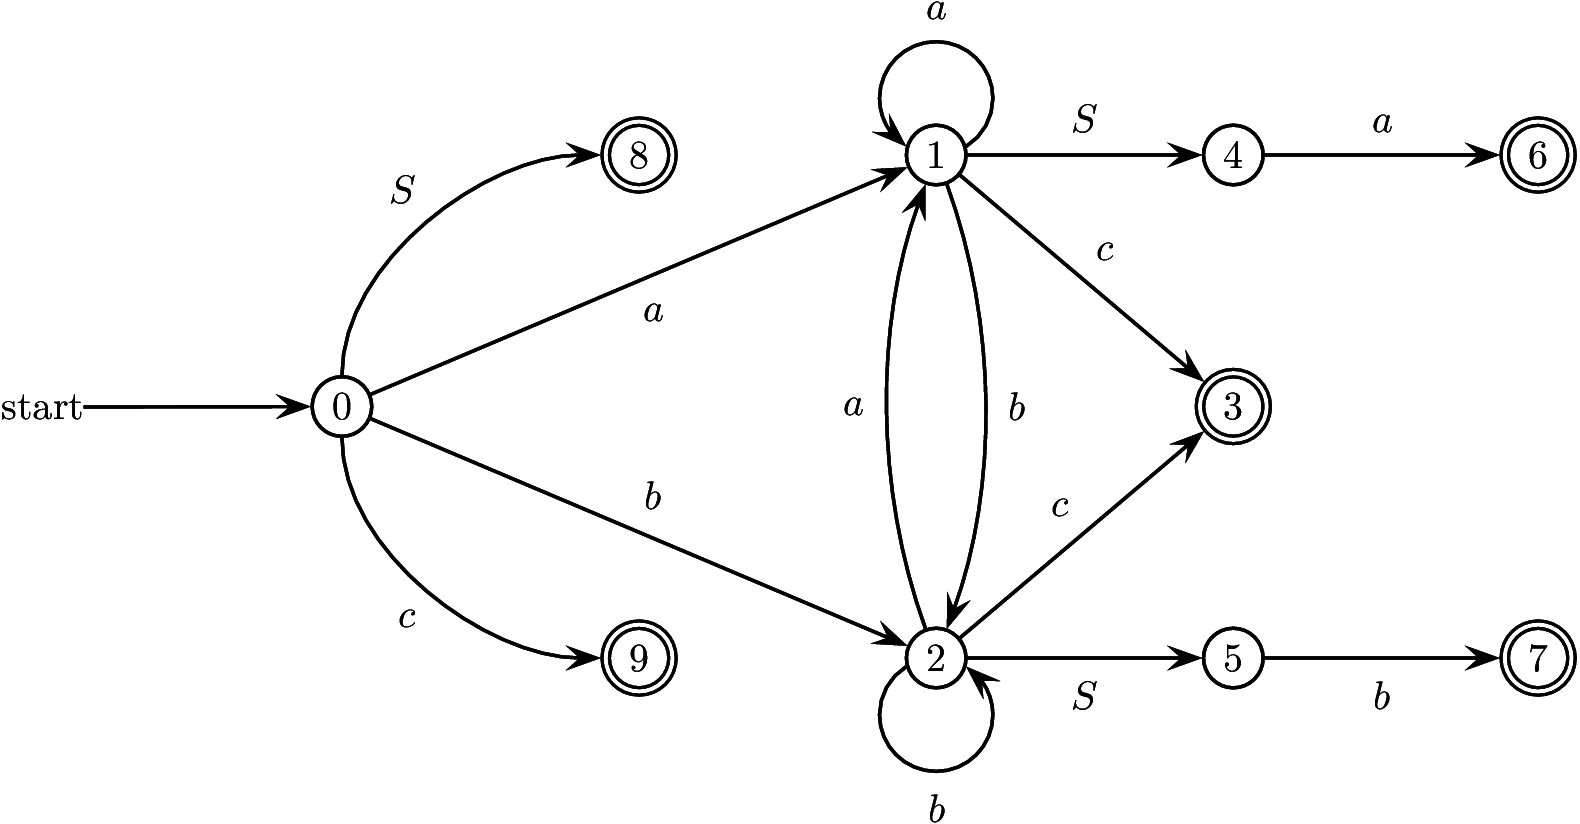
\includegraphics[scale=0.15]{figures/lrparseexamples03.png}
\end{frame}

\sect{LR(1) parsing, a more complex example}

\begin{columns}
\column{0.5\textwidth}
\bee
S \arr aCd \ | \ bCD\\
C \arr cC \ | \ c\\
D \arr d
\eee


\myfig{accdtree}

\column{0.5\textwidth}
\begin{tabular}{|lr|l|}\hline
Stack & Input & Rule \\\hline
\$ & acccd\$ & shift\\
\$a & cccd\$ & shift\\
\$ac & ccd\$ & shift\\
\$acc & cd\$ & shift\\
\$accc & d\$ & C\ar c\\
\$accC & d\$ & C\ar cC\\
\$acC & d\$ & C\ar cC\\
\$aC & d\$ & shift\\
\$aCd & \$ & S \ar aCd\\
\$S & \$ &    accept\\\hline
\end{tabular}

\end{columns}

\bigskip

$S \dar aCd \dar acCd \dar accCd \dar acccd$

\end{frame}

\sect{LR(1) parsing}

\begin{columns}
\column{0.5\textwidth}
\bee
S \arr aCd \ | \ bCD\\
C \arr cC \ | \ c\\
D \arr d
\eee


\myfig{bccdtree}

\column{0.5\textwidth}
\begin{tabular}{|lr|l|}\hline
Stack & Input & Rule \\\hline
\$ & bcccd\$ & shift\\
\$b & cccd\$ & shift\\
\$bc & ccd\$ & shift\\
\$bcc & cd\$ & shift\\
\$bccc & d\$ & C \ar c\\
\$bccC & d\$ & C \ar cC\\
\$bcC & d\$ & C \ar cC\\
\$bC & d\$ & shift\\
\$bCd & \$ & D\ar d\\
\$bCD & \$ & S\ar bCD\\
\$S & \$ &    accept\\\hline
\end{tabular}

\end{columns}

\bigskip

$S \dar bCD \dar bCd \dar bcCd \dar bccCd \dar bcccd$

\end{frame}

\sect{LR(1) parsing}

\bee
S \arr aCd \ | \ bCD\\
C \arr cC \ | \ c\\
D \arr d
\eee


\bi
\li $S \dar aCd \dar acCd \dar accCd \dar acccd$
\li $S \dar bCD \dar bCd \dar bcCd \dar bccCd \dar bcccd$
\li At any point, the derivation string must look like one of these:

\bigskip

$aCd$\hfill $ac^+Cd$\hfill $ac^+d$\hfill $bCD$\hfill $bCd$\hfill
$bc^+Cd$\hfill $bc^+d$

\bigskip

\li Whenever we see one of these, we have to know which rule to apply
at what point in the shifting of the string.
\ei

\end{frame}

\sect{LR(1) parsing}
\small
\begin{columns}
\column{0.4\textwidth}

\bee
S \arr aCd \ | \ bCD\\
C \arr cC \ | \ c\\
D \arr d
\eee

\vspace{1cm}

\begin{tabular}{|lr|l|}\hline
Stack & Input & Rule \\\hline
\$ & acccd\$ & shift\\
\$a & cccd\$ & shift\\
\$ac & ccd\$ & shift\\
\$acc & cd\$ & shift\\
\$accc & d\$ & C\ar c\\
\$accC & d\$ & C\ar cC\\
\$acC & d\$ & C\ar cC\\
\$aC & d\$ & shift\\
\$aCd & \$ & S \ar aCd\\
\$S & \$ &    accept\\\hline
\end{tabular}



\column{0.6\textwidth}

\lrtable

\begin{tabular}{|lr|l|}\hline
Stack & Input & Rule \\\hline
\$ & bcccd\$ & shift\\
\$b & cccd\$ & shift\\
\$bc & ccd\$ & shift\\
\$bcc & cd\$ & shift\\
\$bccc & d\$ & C \ar c\\
\$bccC & d\$ & C \ar cC\\
\$bcC & d\$ & C \ar cC\\
\$bC & d\$ & shift\\
\$bCd & \$ & D\ar d\\
\$bCD & \$ & S\ar bCD\\
\$S & \$ &    accept\\\hline
\end{tabular}

\end{columns}

\end{frame}

\sect{DFA for LR parsing}
\small
\begin{columns}
\column{0.4\textwidth}

\bee
S \arr aCd \ | \ bCD\\
C \arr cC \ | \ c\\
D \arr d
\eee

\column{0.6\textwidth}

\lrtable

\end{columns}
\myfigt{lrdfa}

\end{frame}

\sect{Using the DFA in LR parsing}
\small
\begin{columns}
\column{0.5\textwidth}

\lrtable

\begin{tabular}{|lr|l|}\hline
Stack & Input & Rule \\\hline
0 & acccd\$ & shift\\
0 a 1 & cccd\$ & shift\\
0 a 1 c 4 & ccd\$ & shift\\
0 a 1 c 4 c 4 & cd\$ & shift\\
0 a 1 c 4 c 4 c 4 & d\$ & C\ar c\\
0 a 1 c 4 c 4 C 5 & d\$ & C\ar cC\\
0 a 1 c 4 C 5 & d\$ & C\ar cC\\
0 a 1 C 2 & d\$ & shift\\
0 a 1 C 2 d 3 & \$ & S \ar aCd\\
0 S 12 & \$ &    accept\\\hline
\end{tabular}

\column{0.5\textwidth}
\myfigt{lrdfa}
\end{columns}

\end{frame}

\sect{Using the DFA in LR parsing}
\small
\begin{columns}
\column{0.6\textwidth}

\lrtable


\begin{tabular}{|lr|l|}\hline
Stack & Input & Rule \\\hline
0 & bcccd\$ & shift\\
0 b 6 & cccd\$ & shift\\
0 b 6 c 10 & ccd\$ & shift\\
0 b 6 c 10 c 10 & cd\$ & shift\\
0 b 6 c 10 c 10 c 10 & d\$ & C \ar c\\
0 b 6 c 10 c 10 C 11 & d\$ & C \ar cC\\
0 b 6 c 10 C 11 & d\$ & C \ar cC\\
0 b 6 C 7 & d\$ & shift\\
0 b 6 C 7 d 9 & \$ & D\ar d\\
0 b 6 C 7 D 8 & \$ & S\ar bCD\\
0 S 12 & \$ &    accept\\\hline
\end{tabular}

\column{0.5\textwidth}
\myfigt{lrdfa}
\end{columns}

\end{frame}

\sect{More examples in notes on repo.}
\end{frame}

\sect{LR(k) languages, Knuth's theorem}

\begin{theo}
\bee LR(k) \mbox{~languages~} &=& LR(1) \mbox{~languages~}\\
 &=& \mbox{deterministic context free languages}
\eee
\end{theo}
\end{frame}

\sect{LR parsing exercises}

Redo all the solved examples.  Also,
find DFAs and tables for the following languages, and trace some
parses:
\bi
\li $S \ar a \mid b \mid c$
\li $S \ar aSa \mid b$
\li $S \ar ABC $\\
$A\ar a$\\$B\ar b$\\$C\ar c$
\ei
\end{frame}

\end{document}
